\section{Homework 2}

\subsection{Il problema}
Come secondo homework si affronta il classico \textit{gambler's problem}. Un giocatore possiede una certa somma di denaro e, a ogni turno, scommette su un lancio di una moneta un importo a sua scelta, purché non superiore al capitale posseduto. Se vince, il capitale aumenta dell'importo scommesso; se perde, il capitale diminuisce dello stesso importo. Il gioco termina quando il giocatore raggiunge $100$ (obiettivo) oppure quando resta senza soldi (rovina): in entrambi i casi lo stato è assorbente. La reward è $0$ per ogni transizione intermedia, $+1$ quando si raggiunge l'obiettivo e $-1$ quando si finisce in rovina.

Il modello è definito nel file \code{modelGambler.m}, dove vengono costruite la matrice delle probabilità di transizione $P$ e la matrice delle ricompense attese $R$, indicizzate su stati (capitale posseduto, da $0$ a $100$) e azioni (importo scommesso). Queste due strutture sono l'input necessario per applicare gli algoritmi di \textit{Dynamic Programming}.

\begin{infobox}[Parametri]
\begin{itemize}[nosep]
    \item Probabilità di vittoria della moneta: $p = 0.50$ 
    \item Fattore di sconto: $\gamma = 0.99$ 
\end{itemize}
\end{infobox}

\subsection{Algoritmi}
Per risolvere il problema si sono utilizzati due algoritmi di \textit{Dynamic Programming}: \textit{Policy Iteration} e \textit{Value Iteration}, entrambi basati sulla conoscenza completa di $P$ e $R$.

\paragraph{Policy Iteration.} L'algoritmo alterna due fasi fino a convergenza della policy:
\begin{itemize}[nosep]
    \item \emph{Policy evaluation}: calcolo della funzione valore $V_\pi$ per la policy corrente, iterando fino a convergenza tramite la Bellman Expectation Equation;
    \item \emph{Policy improvement}: aggiornamento della policy rendendola greedy rispetto alla $V_\pi$ appena calcolata.
\end{itemize}
Le due fasi si ripetono finché la policy non cambia più tra un'iterazione e la successiva.

\paragraph{Value Iteration.} A differenza della policy iteration, non viene mai calcolata esplicitamente una policy intermedia: a ogni iterazione si aggiorna direttamente $V$ tramite la Bellman Optimality Equation
\[
V(s) \leftarrow \max_{a} \sum_{s'} P(s'\mid s,a)\big[R(s,a) + \gamma V(s')\big]
\]
finché $V$ non converge. La policy ottima si ricava, solo alla fine, rendendola greedy rispetto alla $V$ così ottenuta.

La differenza sostanziale tra i due algoritmi è quindi nel ruolo della policy durante il calcolo: nella policy iteration $V$ viene sempre valutata rispetto a una policy esplicita, che viene poi migliorata; nella value iteration $V$ viene aggiornata direttamente verso il suo valore ottimo, senza passare per una policy intermedia. Questo rende le singole iterazioni della value iteration più leggere, ma può richiedere un numero di iterazioni maggiore per convergere rispetto alla policy iteration.

\subsection{Risultati}
Le simulazioni sono state condotte prima nel caso di moneta equa ($p = 0.50$), variando il fattore di sconto $\gamma \in \{0.99,\ 0.90,\ 0.4\}$, e poi nel caso di moneta truccata, rispettivamente con $p = 0.4,\ \gamma = 0.99$ e con $p = 0.55,\ \gamma = 0.999$. Per il confronto si utilizza il grafico della funzione $Q(s,a)$, sovrapposto alla policy trovata $\pi(s)$ (linea rossa), poiché $Q$ è più informativa di $V$: permette infatti di visualizzare, per ogni stato, quali azioni sono ottime (o quasi ottime), e non solo il valore dello stato migliore.

\subsubsection*{Caso $p = 0.50$}

Nel caso $\gamma = 0.99$ (figura \ref{fig:1_h2}) si nota che, per ogni capitale $s$, la funzione $Q(s,a)$ è pressoché costante al variare della scommessa $a$, purché $a \le \min(s, 100-s)$. Questo non è un caso: con moneta equa, la probabilità di raggiungere l'obiettivo prima della rovina dipende, per un risultato classico della teoria della rovina del giocatore, esclusivamente dal capitale $s/100$, indipendentemente dall'importo scommesso a ogni turno. Tutte le azioni $a \le \min(s,100-s)$ sono quindi \emph{esattamente} equivalenti, ed è per questo che la forma triangolare della policy trovata è in buona parte casuale: rappresenta una sola fra le infinite policy ottime possibili, non l'unica, e la scelta specifica dipende soltanto da come l'operazione di $\max$ rompe il pareggio tra azioni. Questo spiega anche perché la policy individuata dalla value iteration, pur convergendo allo stesso $V^*$ della policy iteration, oscilli in modo irregolare attorno alla soluzione "a scalini" trovata dalla policy iteration: trattandosi di azioni realmente equivalenti in termini di $Q$, bastano errori numerici trascurabili perché l'operazione di $\max$ selezioni un'azione diversa da uno stato al successivo.

Aumentando $\gamma$ (confrontando le figure \ref{fig:3_h2}, \ref{fig:2_h2} e \ref{fig:1_h2}, con $\gamma = 0.4,\ 0.90,\ 0.99$) questo pareggio tra le azioni diventa via via più netto: al crescere di $\gamma$ verso $1$ il numero di scommesse necessarie per terminare la partita viene scontato sempre meno, e quindi $Q(s,a)$ smette di dipendere dalla velocità con cui si raggiunge l'obiettivo, riavvicinandosi al caso teorico in cui tutte le $a\le\min(s,100-s)$ sono identiche. Con $\gamma$ più basso, invece, terminare la partita in meno mosse viene premiato (scontato di meno), per cui le scommesse più alte iniziano a essere leggermente preferite rispetto a quelle più basse: il pareggio non è più perfetto, ed è per questo che con $\gamma=0.4$ la value iteration mostra una policy ancora più rumorosa, oscillando attorno a un ottimo che comincia ad assomigliare a quello, unico, del caso sfavorevole discusso di seguito.


\subsubsection*{Caso $p = 0.4$ e $p = 0.55$}
Per verificare che i due algoritmi individuino la stessa soluzione ottima anche quando la moneta non è equa, sono stati testati anche i casi $p = 0.4,\ \gamma = 0.99$ (figura \ref{fig:4_h2}) e $p = 0.55,\ \gamma = 0.999$ (figura \ref{fig:5_h2}). In entrambi i casi le policy trovate dai due metodi coincidono, confermando la correttezza delle due implementazioni.

A differenza del caso equo, con $p = 0.55$ (moneta favorevole al giocatore) la funzione $Q(s,a)$ non è più pressoché costante: cresce nettamente al diminuire della scommessa, per ogni capitale. La policy ottima diventa quindi unica e ben definita, e consiste nello scommettere il minimo possibile: moltiplicando il numero di lanci si sfrutta al meglio il vantaggio atteso positivo per lancio, riducendo il rischio legato alla varianza di poche scommesse grandi.

Con $p = 0.4$ (moneta sfavorevole), a $\gamma = 0.99$ la policy trovata segue, in apparenza, lo stesso confine triangolare $a = \min(s,100-s)$ visto nel caso equo. La differenza sostanziale, però, è che qui quel confine \emph{non} è più uno fra tanti ottimi equivalenti, ma è l'unica policy ottima: con una moneta sfavorevole ($p<0.5$), ridurre il numero di scommesse necessarie a decidere l'esito della partita è strettamente vantaggioso, e la strategia \emph{bold} di scommettere il massimo possibile ($\min(s,100-s)$, per non superare l'obiettivo) è l'unica a massimizzare la probabilità di raggiungere $100$ prima della rovina. Ogni scommessa più bassa è quindi strettamente peggiore, anche se la scala di colori della figura, dominata dai valori negativi vicini allo zero, non rende evidente a colpo d'occhio questa differenza.
\subsubsection*{Diminuire $\gamma$}
In tutti i casi la diminuzione del fattore di sconto $\gamma$ rende la funzione $Q(s,a)$ sempre piu uniforme, fino a raggiungere un valore quasi costante per ogni coppia di $s,a$. Questo chiaramente non è un problema per il caso $p=0.5$, dove si è visto che ogni policy sia equivalente a quella ottimale, e non lo è nemmeno per il caso $p<0.5$, dove il banco ha il vantaggio e il gioco al lungo andare sfavorisce il giocatore, invece un gioco breve lo ricompense. Pero è un grande problema per il caso $p>0.5$, dove la policy ottimale puo essere trovata solo per valori di $\gamma$ alti.

\begin{figure}[htbp]
    \centering
    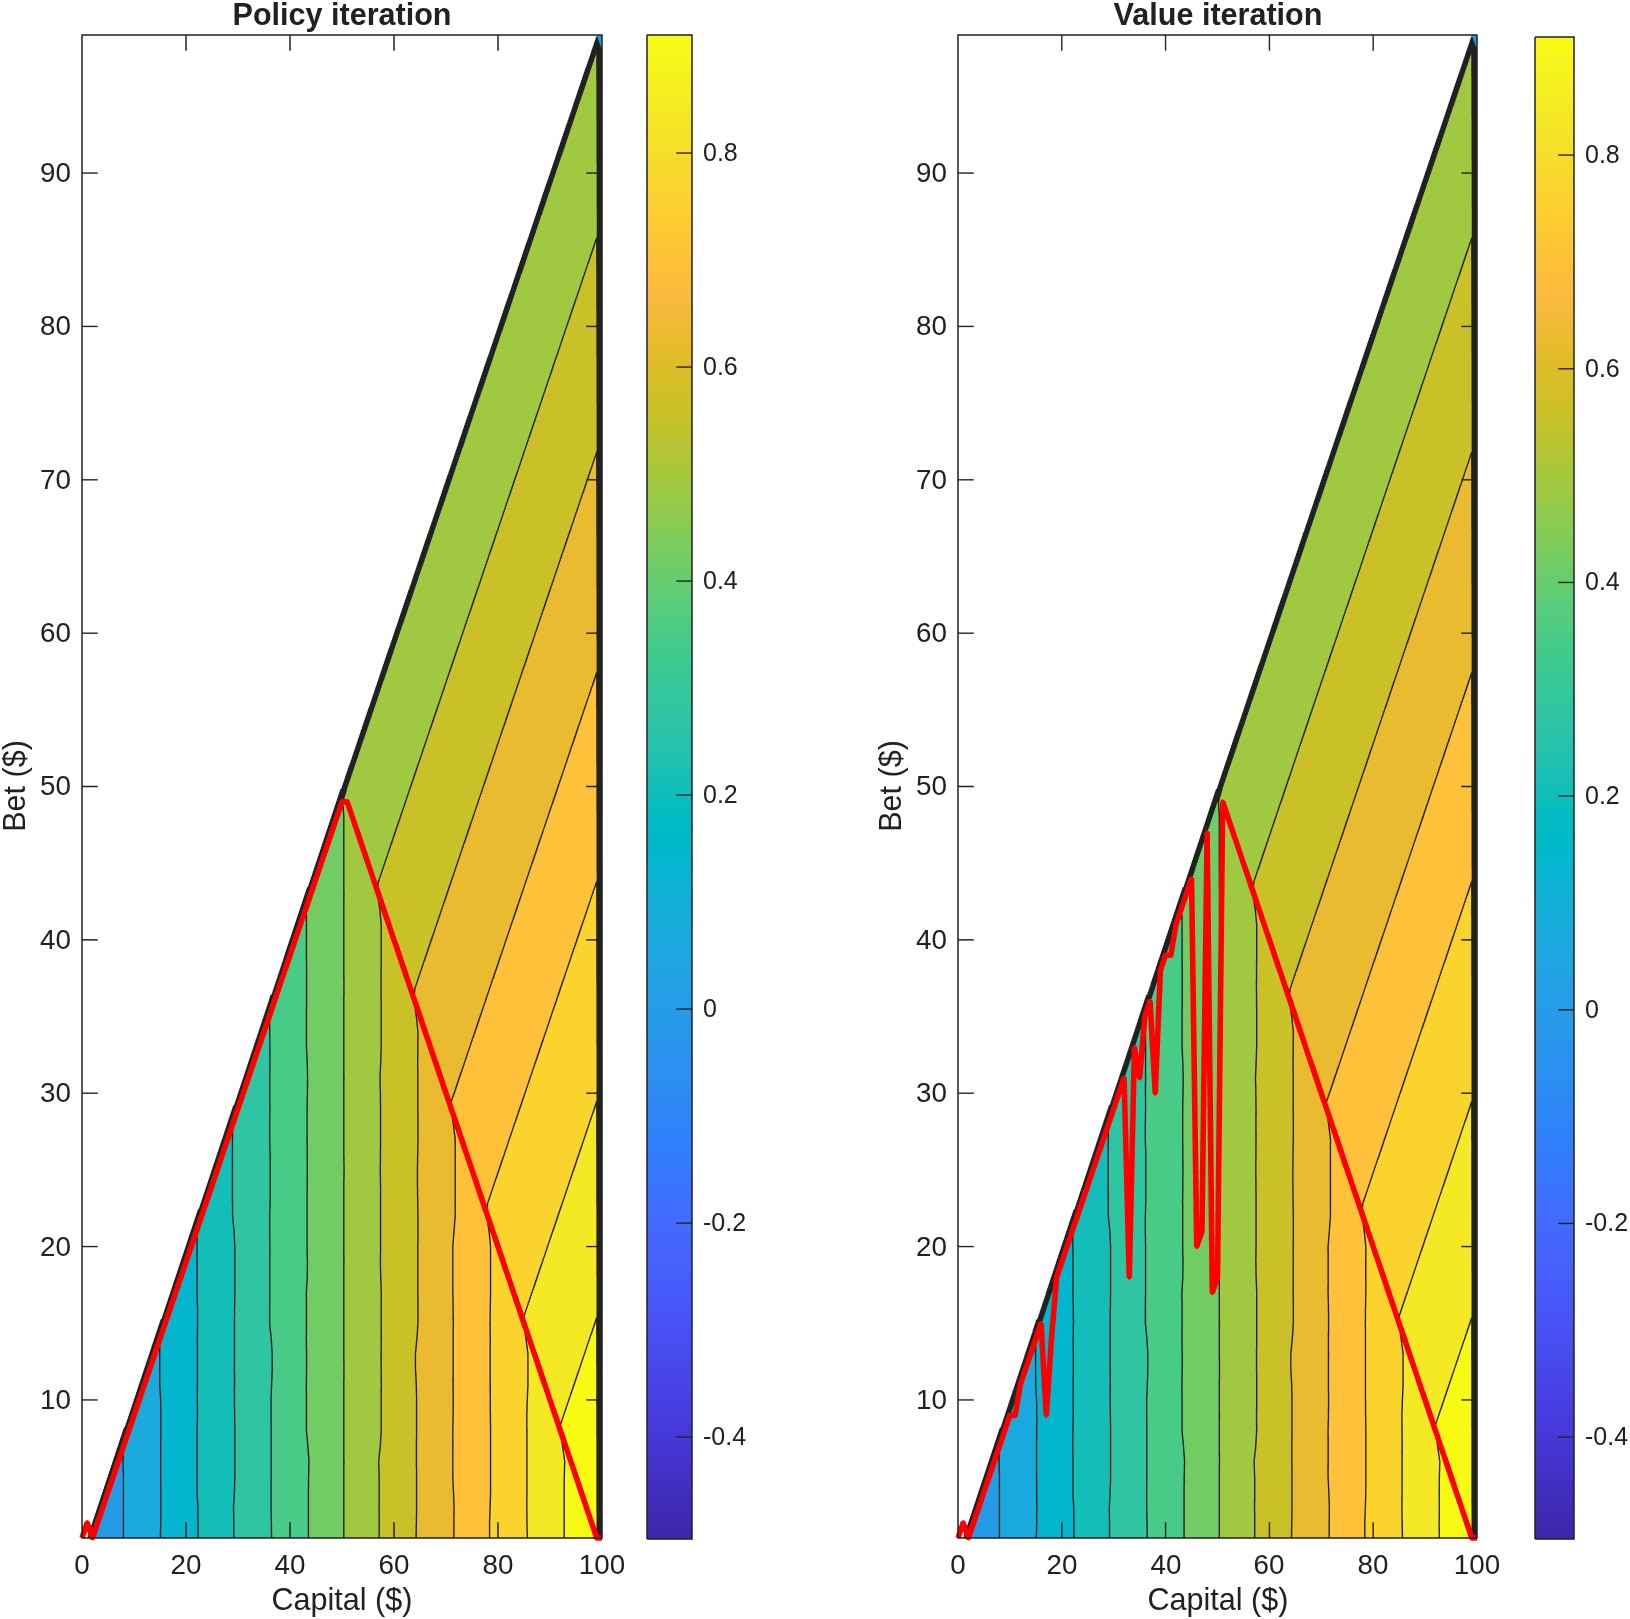
\includegraphics[width=1\textwidth]{homeworks/2/img/5_99.jpg}
    \caption{p = 0.50, $\gamma$ = 0.99}\label{fig:1_h2}
\end{figure}
\begin{figure}[htbp]
    \centering
    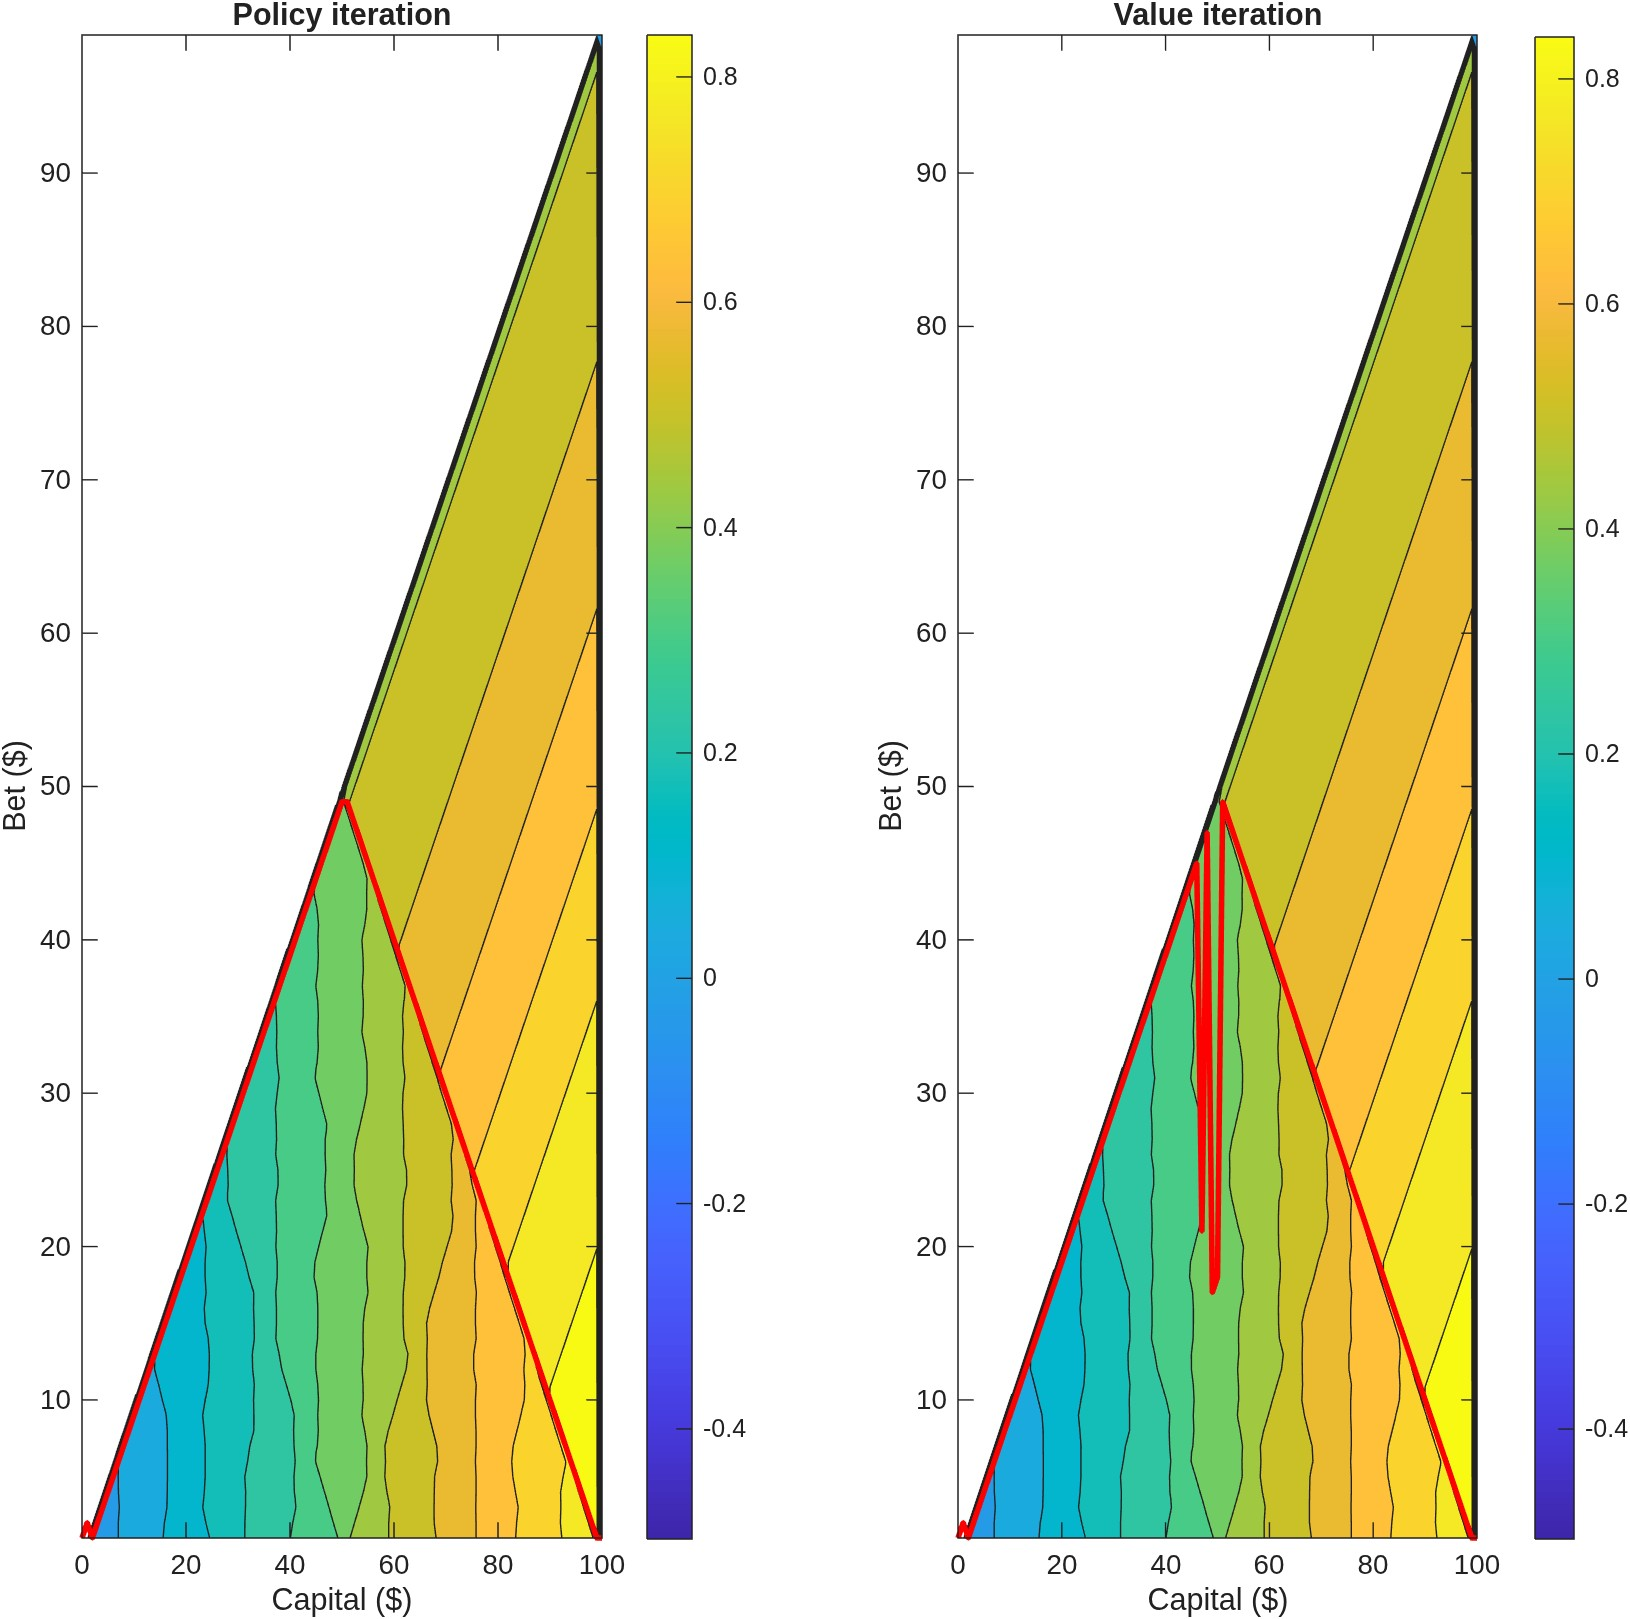
\includegraphics[width=1\textwidth]{homeworks/2/img/5_9.jpg}
    \caption{p = 0.50, $\gamma$ = 0.90}\label{fig:2_h2}
\end{figure}
\begin{figure}[htbp]
    \centering
    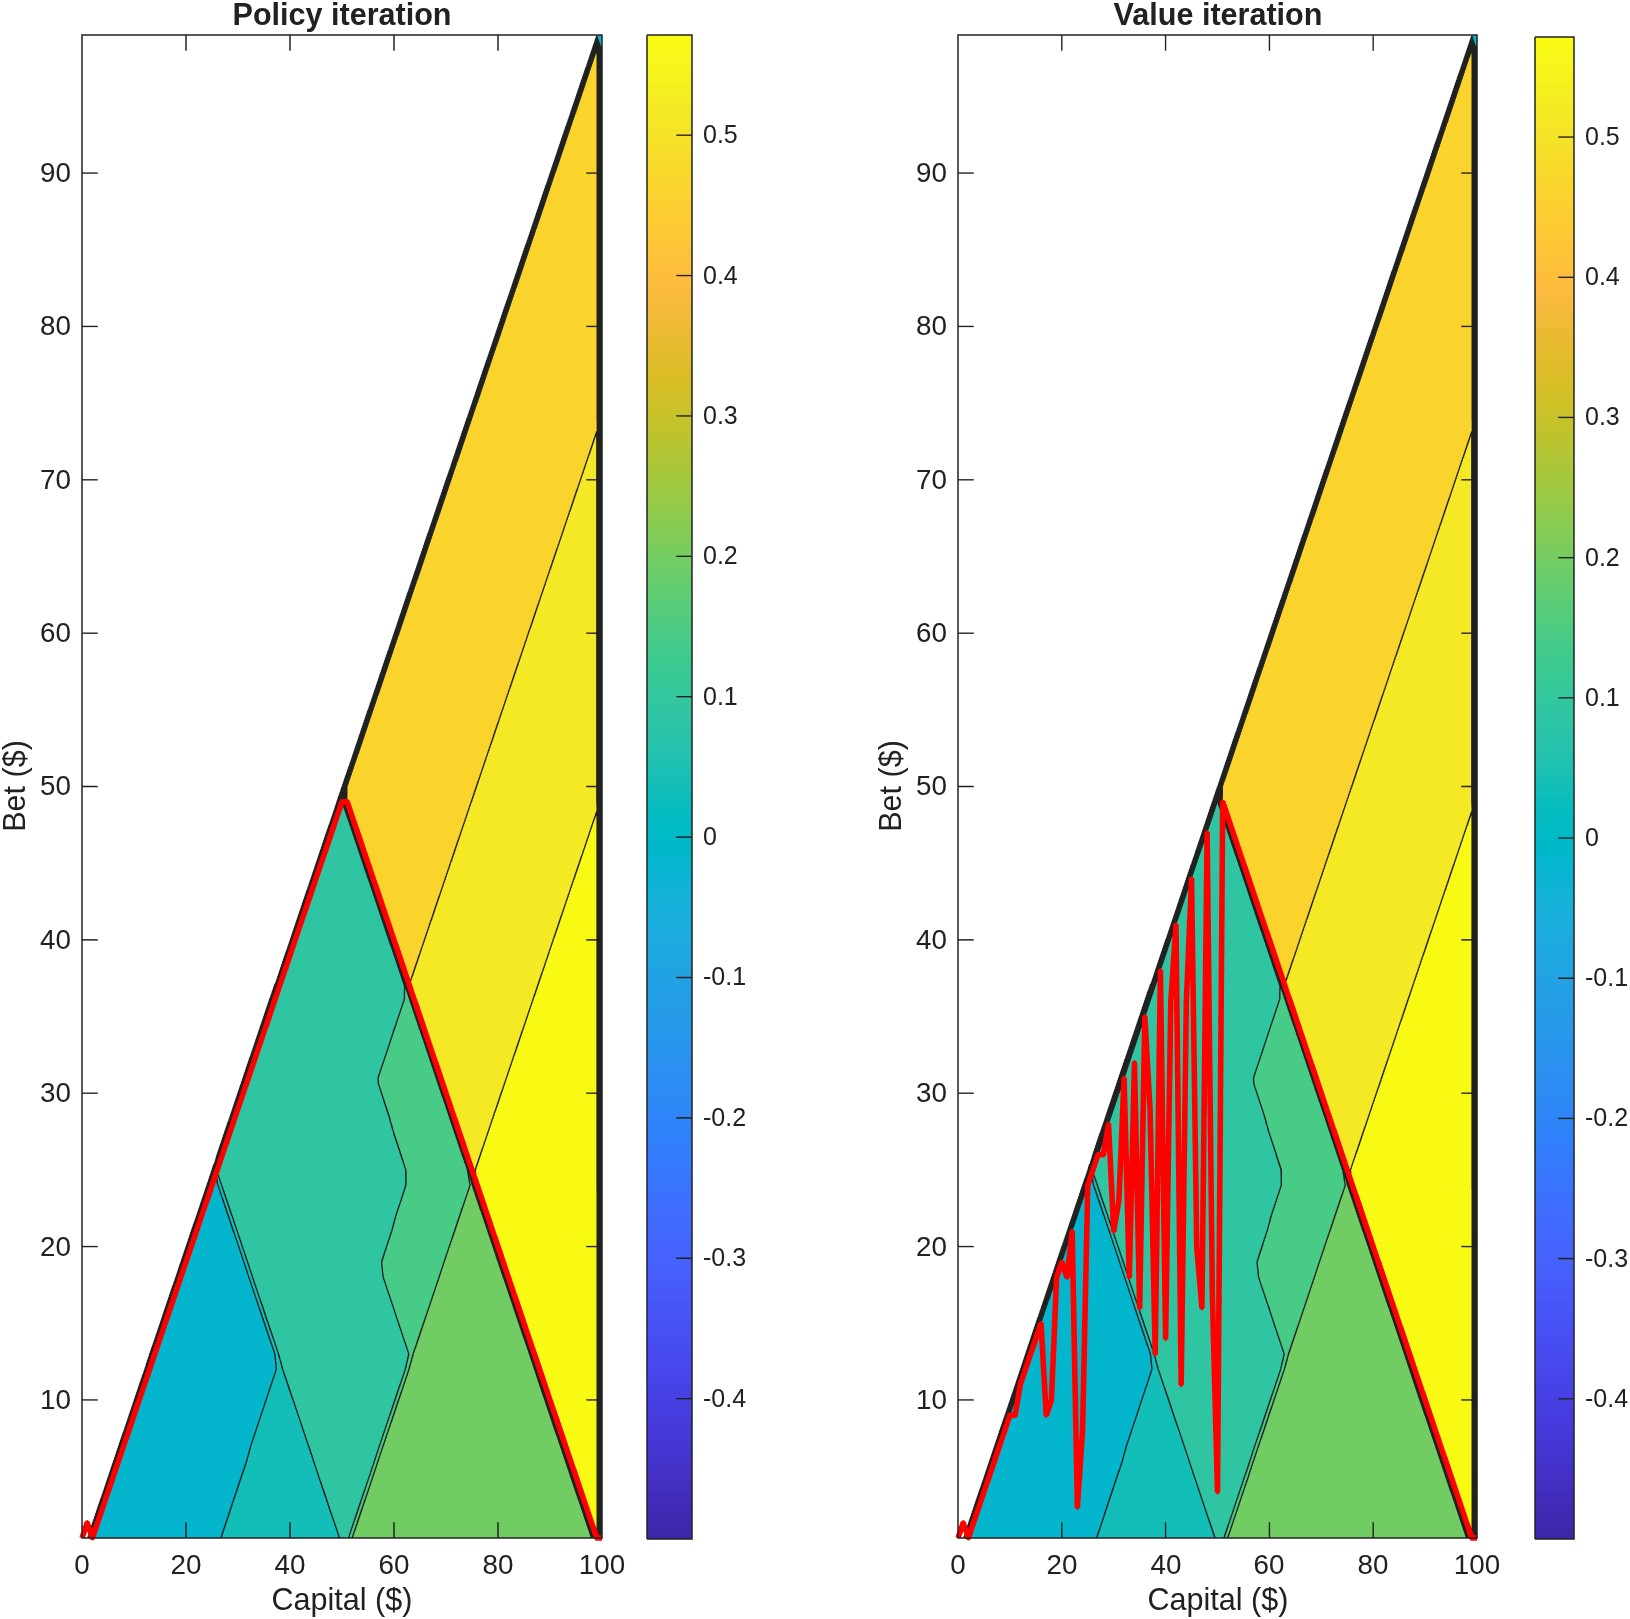
\includegraphics[width=1\textwidth]{homeworks/2/img/5_4.jpg}
    \caption{p = 0.50, $\gamma$ = 0.4}\label{fig:3_h2}
\end{figure}


\begin{figure}[htbp]
    \centering
    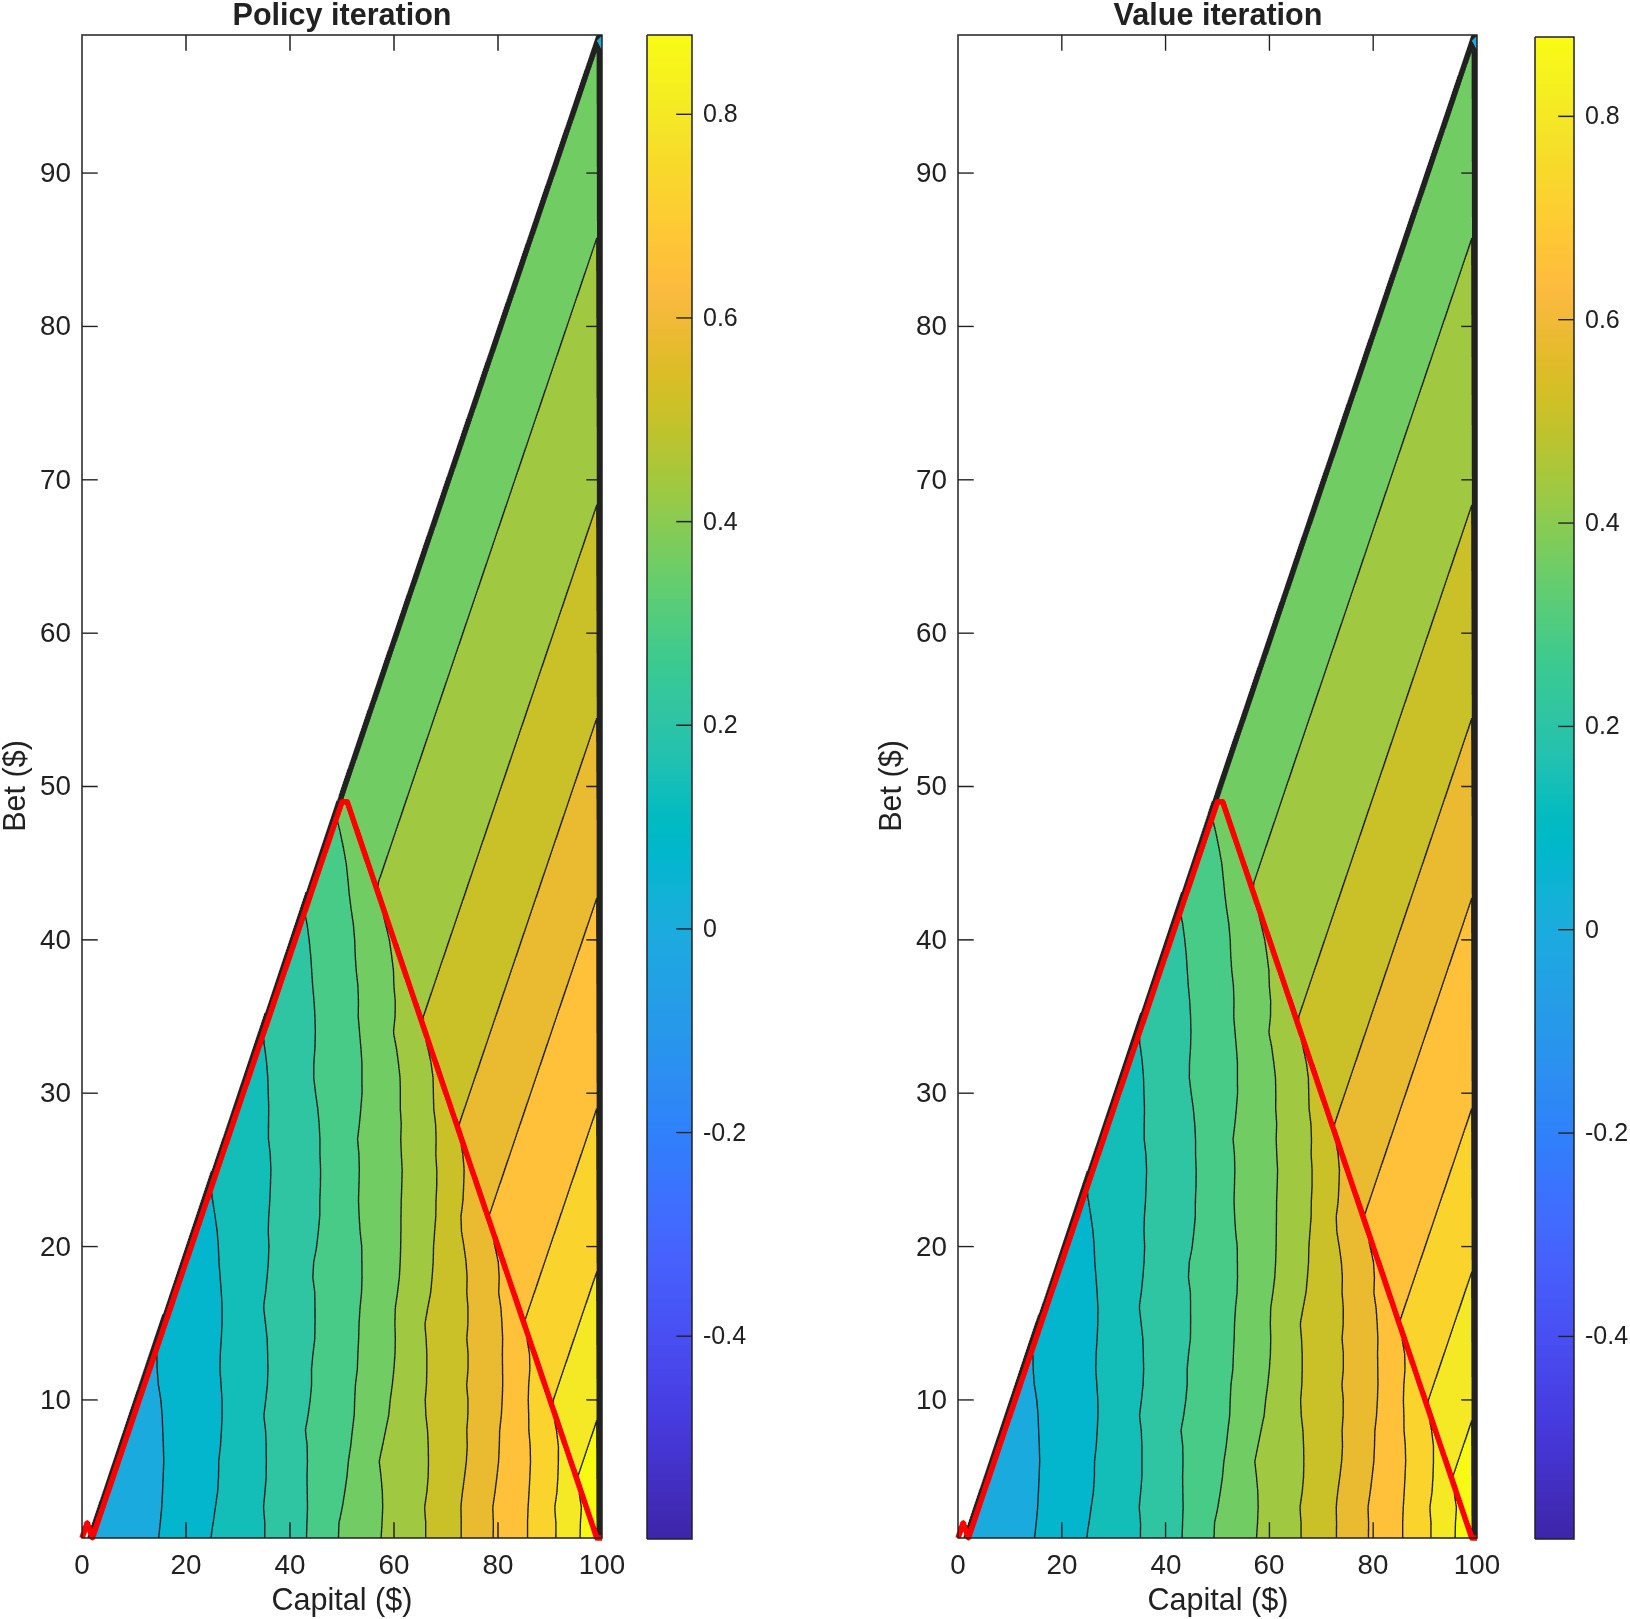
\includegraphics[width=1\textwidth]{homeworks/2/img/4_99.jpg}
    \caption{p = 0.4, $\gamma$ = 0.99}\label{fig:4_h2}
\end{figure}
\begin{figure}[htbp]
    \centering
    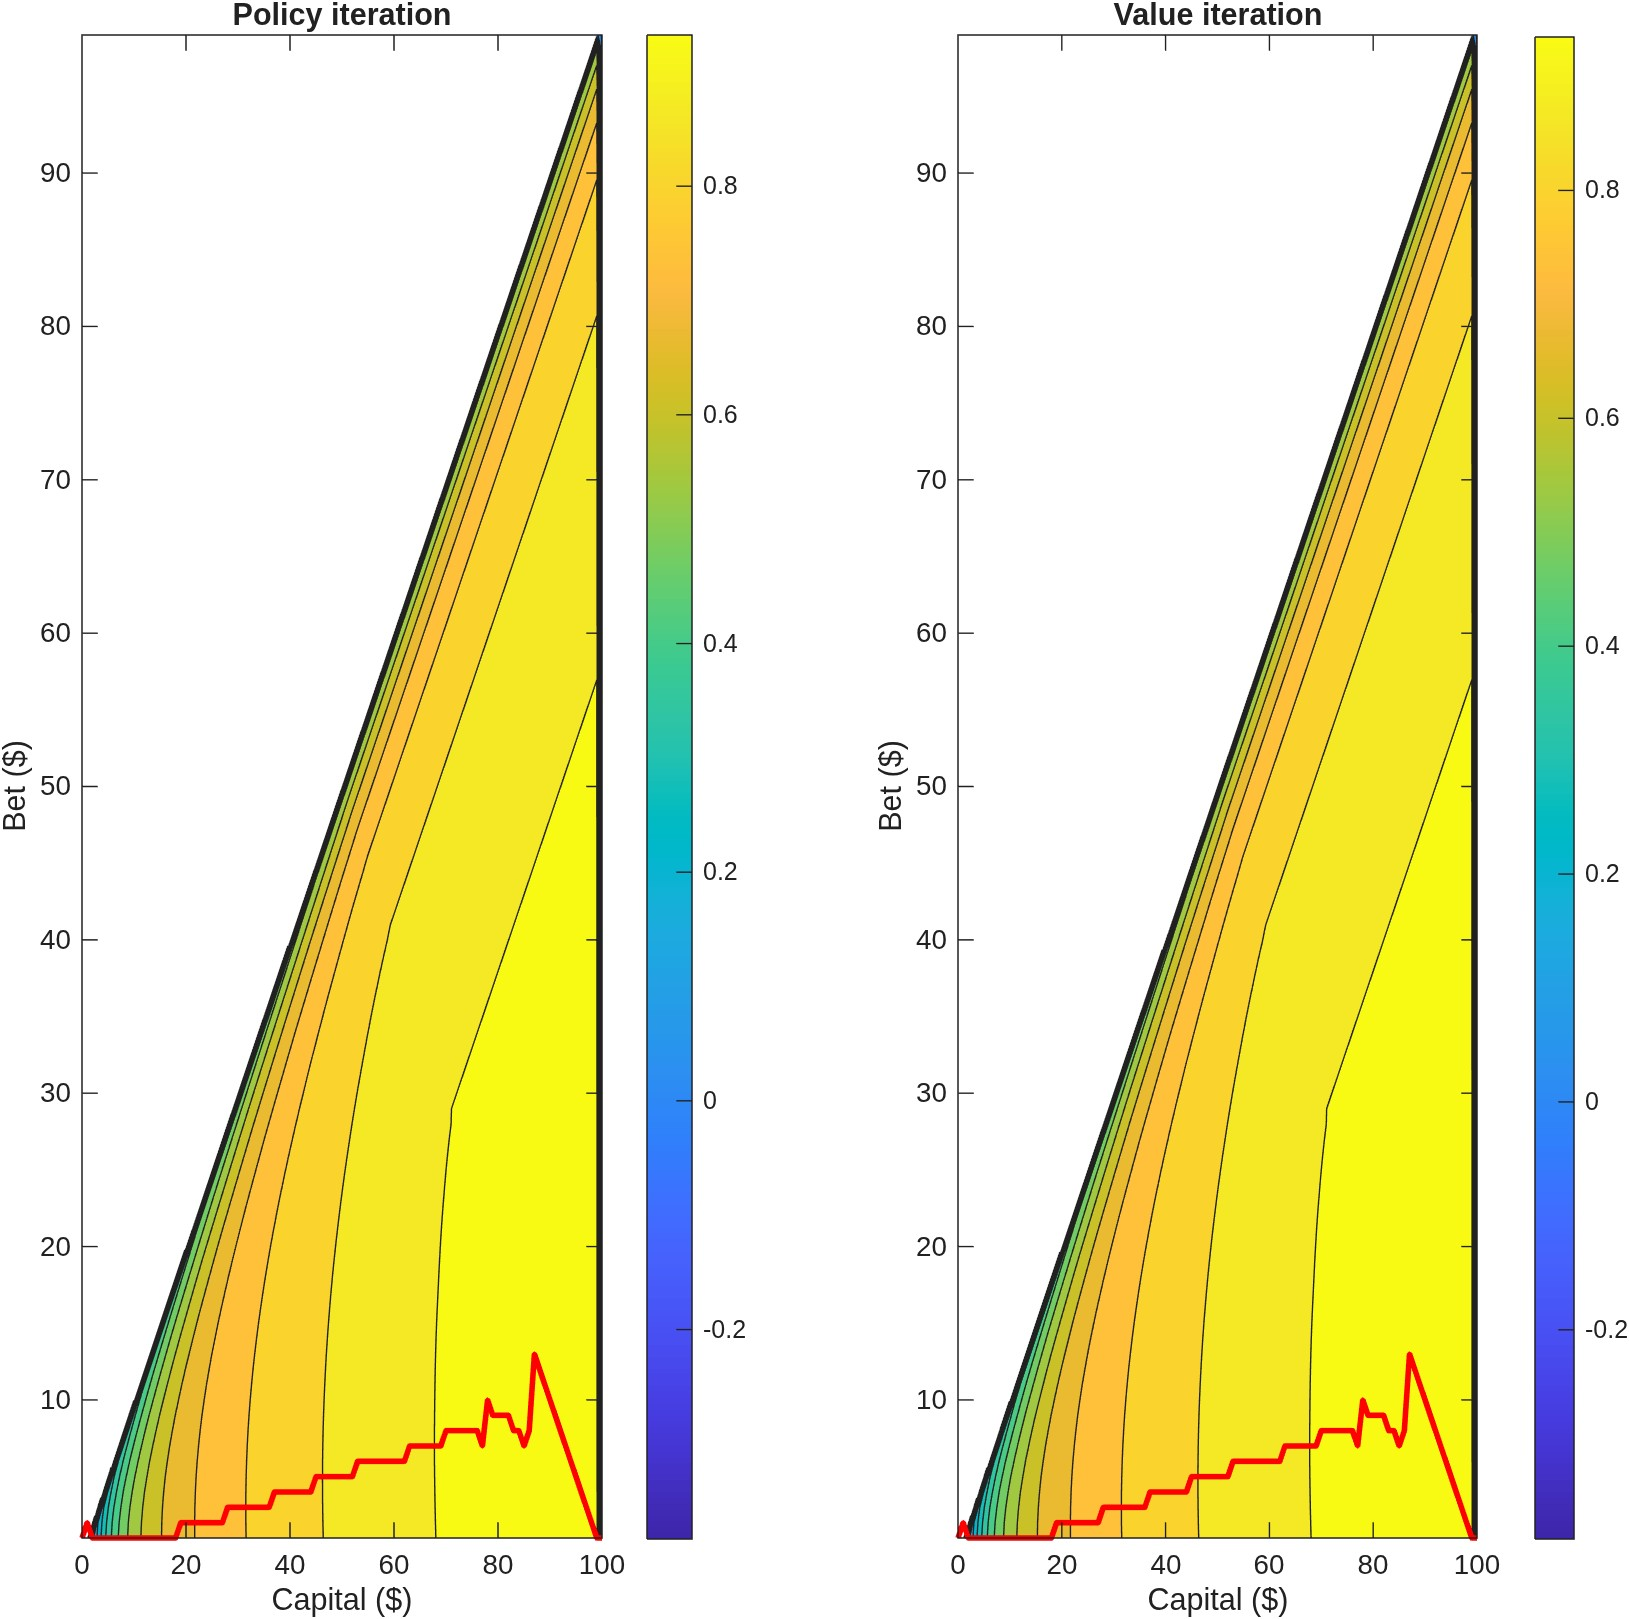
\includegraphics[width=1\textwidth]{homeworks/2/img/55_999.jpg}
    \caption{p = 0.55, $\gamma$ = 0.999}\label{fig:5_h2}
\end{figure}